\hypertarget{5}{}

\rhead{K-RET: Knowledgeable Biomedical Relation Extraction System}
\lhead{Chapter 5}

\chapter[K-RET: Knowledgeable Biomedical Relation Extraction System]
{\huge K-RET: Knowledgeable Biomedical Relation Extraction System \\
\Large \textmd{Diana F. Sousa and Francisco M. Couto}}

\vspace{-1.6cm}

% Gray Line
\begingroup
\color{black}
\par\noindent\rule{\textwidth}{0.4pt}
\endgroup

\noindent{This chapter tackles Objective 1 by integrating knowledge to expand text training data of BERT-based models. This work is particularly relevant to tackle the main hypothesis of this thesis since it is the most recent and includes all expertise acquired throughout the doctoral work. Corresponds to the journal article:} 

\begin{itemize}[label=]
    \item{\textbf{Sousa, D. F.} and Couto, F. M. (2023). \textbf{K-RET: Knowledgeable Biomedical Relation Extraction System}. Bioinformatics, 39(4):1-8. (Q1 Scimago) \citep{sousa2023k}}
\end{itemize}

\textbf{Abstract.} \textbf{Motivation:} Relation Extraction (RE) is a crucial process to deal with the amount of text published daily, for example, to find missing associations in a database. RE is a text mining task for which the state-of-the-art approaches use bidirectional encoders, namely, BERT. However, state-of-the-art performance may be limited by the lack of efficient external knowledge injection approaches, with a larger impact in the biomedical area given the widespread usage and high quality of biomedical ontologies. This knowledge can propel these systems forward by aiding them in predicting more explainable biomedical associations. With this in mind, we developed K-RET, a novel, knowledgeable biomedical relation extraction system that, for the first time, injects knowledge by handling different types of associations, multiple sources and where to apply it, and multi-token entities.\\
\textbf{Results:} We tested K-RET on three independent and open-access corpora (DDI, BC5CDR, and PGR) using four biomedical ontologies handling different entities. K-RET improved state-of-the-art results by 2.68\% on average, with the DDI Corpus yielding the most significant boost in performance, from 79.30\% to 87.19\% in F-measure, representing a p-value of $2.91 \times 10^{-12}$.\\
\textbf{Availability:} \url{https://github.com/lasigeBioTM/K-RET}

\section{Introduction}

With the exponential increase in the number of research articles published in the last decades, researchers find it hard to keep up with all relevant information for their respective fields. The overwhelming number of research papers, particularly in the biomedical field, frequently makes it impossible for researchers and clinicians to be aware of all established entity associations and dissociations. This unawareness often leads to experimental repetition to prove or disprove hypotheses already studied. Further, even if the hypothesis is unique or new, the same inference could often be retrieved from knowledge about experiments done on similar entities. Automated biomedical Relation Extraction (RE) is a fundamental step toward aiding these researchers and clinicians in saving time and focusing their work on genuinely novel associations.

Through the years, several approaches have been employed to tackle biomedical RE, from straightforward rule-based approaches \citep{rinaldi2007mining,kilicoglu2020broad} to entire machine learning dedicated systems \citep{houssein2021machine,abdelkader2021machine}, in which deep learning played a significant role \citep{dash2020deep}. Successively, these approaches became more specialized in targeting multiple types of biomedical associations from protein-protein relations \citep{kim2006biocontrasts} to human phenotype-gene causality \citep{song2019leveraging,sousa2022biomedical}. BERT \citep{devlin2019bert} and their domain derivatives, such as BioBERT \citep{lee2020biobert}, SciBERT \citep{scibert}, and PubMedBERT \citep{gu2021domain} are the current state-of-the-art employed solutions. They not only successfully extract multiple types of relations from the text but can also, using their pre-trained models, be easily integrated into newer systems targeting different Natural Language Processing (NLP) tasks, such as Named-Entity Recognition (NER) \citep{nasar2021named}, Named-Entity Linking (NEL) or Normalization \citep{ruas2022nilinker}, and Question Answering (QA) \citep{do2022developing}.

However, there are some caveats for most biomedical RE systems. The first limitation is their focus and specialization on one specific type of association \citep{hu2021survey}, with some notable exceptions that are flexible to target more than one type \citep{song2019leveraging,sousa2020biont,sousa2022biomedical}. The second limitation is that systems' results frequently lack an explanation. One can not easily understand how a relation was found and what inferences a particular model made to reach an output. Finally, in close connection with making systems explainable, the third more relevant limitation is their general disregard for the vast repertoire of biomedical dedicated knowledge bases, particularly in the form of ontologies. This multitude of organized biomedical knowledge is freely available, but most systems still rely only on the information from the training data. Some exemptions recently made some strides into using knowledge in the general domain \citep{liu2020k} and the biomedical/clinical domain \citep{hao2020enhancing}. However, these are still limited in the domain's specificity and inflexible to adding different or more structured knowledge.  

Some of the most notary examples of organized biomedical knowledge are the Gene Ontology (GO) \citep{ashburner2000gene,gene2019gene}, the Human Phenotype Ontology (HPO) \citep{kohler2021human}, the Human Disease Ontology (DO) \citep{schriml2022human}, the Chemical Entities of Biological Interest (ChEBI) \citep{degtyarenko2007chebi}, and the Unified Medical Language System (UMLS) \citep{bodenreider2004unified}. Respectively, these organized resources described connections between gene function descriptors, human phenotypes, human diseases, chemicals of biological interest, and clinical entities. 

The work of \cite{liu2020k} is a recent and successful attempt
 for knowledge incorporation into multiple open and specific-domain tasks. Their K-BERT system was able to incorporate domain knowledge without creating a heterogeneous embedding space. The novelty in their approach is the creation of a knowledge layer that injects knowledge directly into the sentence. Then, they perform sentence tree re-arrangement before the embedding layer, with the addition of a soft-position embedding and a visible matrix to target possible readability problems from the re-arrangement. Also, it does not require pre-training of the BERT models it supports, making it suitable for users with limited computational resources \citep{zhao2019uer}. However, their system has some major constrictions. First, the authors do not apply their approach to the RE task for the open or biomedical-specific domains. Second, the knowledge injection can only be used for single tokens within the sentence tree, making it miss knowledge associated with multi-token entities that are most prevalent in the biomedical domain. Third, the application of their system only allows for the injection of knowledge from one knowledge source, constraining data that intersects one or more domains (e.g., patient case reports that mention both the procedures done and the phenotypes associated with the patients). Finally, there is no possibility of injecting target knowledge into the entities of interest; one must always apply knowledge to all possible sentence tokens.   

In this work, we designed a new approach to knowledge injection that is able to address the challenges stated in the last paragraph to create K-RET, a knowledgeable biomedical RE BERT-based system. K-RET is a flexible biomedical RE system, allowing for the use of any pre-trained BERT-based system (e.g., SciBERT and BioBERT) to inject knowledge in the form of knowledge bases from a single source or multiple sources simultaneously. This knowledge can be applied to various contextualizing tokens or just to the tokens of the candidate relation for single and multi-token entities. 

K-RET effectively improves the performance of baseline biomedical BERT-based models by an average of 2.68\% on all datasets (DDI \citep{herrero2013ddi,segura2014lessons}, BC5CDR \citep{li2016biocreative}, and PGR-crowd \citep{sousa2019silver,sousa2020hybrid} Corpora). The most successful configuration is applying contextualised knowledge by adding two knowledge base entities per possible domain entity within each sentence tree (i.e., DDI Corpus plus ChEBI). This work resulted in the following main contributions:\vspace*{1pt}

\begin{itemize}
\item K-RET, a knowledgeable biomedical RE system that allows for the integration of any pre-trained BERT-based system.
\item Approach to flexible injection of knowledge with multi-options:
\begin{enumerate}
    \item association of knowledge to single or multi-token entities in the sentence tree;
    \item add more than one knowledge source to inject knowledge of different domains;
    \item injection of knowledge into targeted or multiple contextualizing tokens in a sentence tree. \vspace*{1pt} 
\end{enumerate}
\end{itemize}

In the following section, System and Methods, we describe K-RET, formally presenting the main architectural features. In Section 3, Implementation, we describe the resources used (datasets and knowledge bases), parameters, training details and the main results of different system configurations. These configurations are the baseline (i.e., without knowledge) and the use of target versus contextualized knowledge within three different biomedical RE datasets. Sections 4 and 5 discuss the previous results with targeted ablation studies and present the main conclusions and future work. 


\section{System and Methods}

In this section, we will present our system K-RET, represented in Figure \ref{fig:51}. We will describe each new system component and how they differ from the implementations from both BERT \citep{devlin2019bert} and K-BERT \citep{liu2020k}, which was built using the UER platform \citep{zhao2019uer}, starting by defining the general Notation and then detailing our additions in Architecture.   

\begin{figure}[hbt!]
\centerline{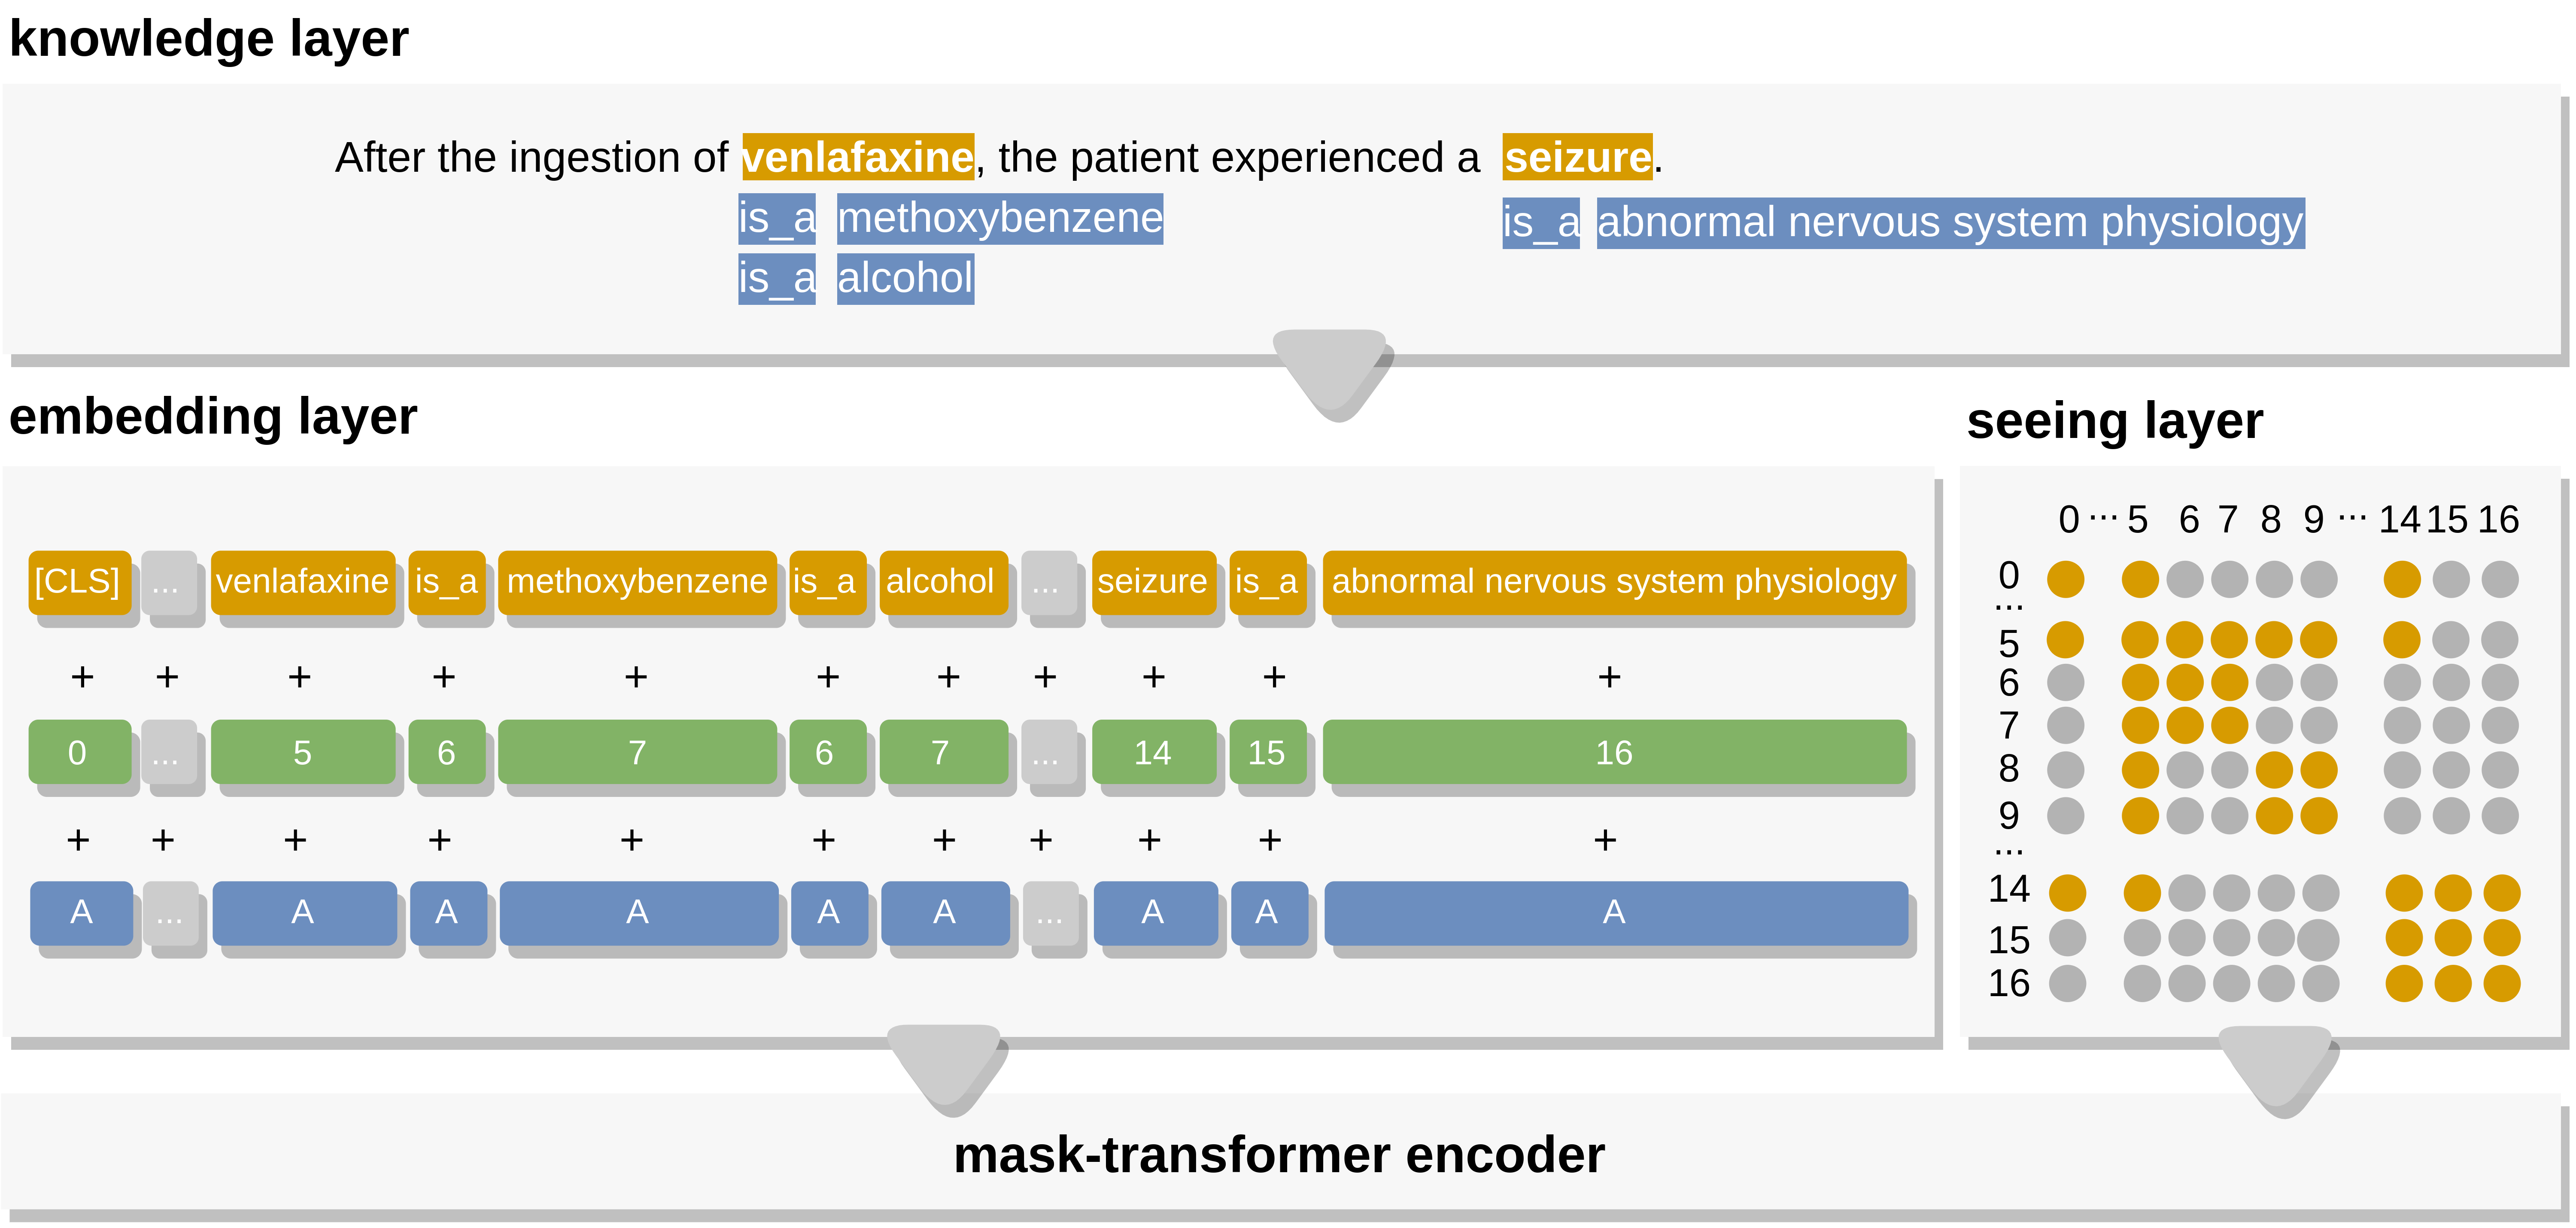
\includegraphics[width=\linewidth]{images/chapter_5/kret_methodology.png}}
\caption[Structured Layer Representation of K-RET]{The structured layer representation of K-RET. In the pipeline, we retrieved a sentence from a biomedical relation extraction dataset with delimited target entities: venlafaxine and seizure. We added a Knowledge layer to these entities from associations made with their respective domain ontologies, the Chemical Entities of Biological Interest (ChEBI) and the Human Disease Ontology (DO). In the Embedding layer, the tokens are flattened into a sequence for token embedding. Then, the soft-position embedding is used along with the token embedding, and the tokens are tagged with A for segment embedding. The orange circles correspond to visible tokens in the Seeing layer, while the grey circles correspond to invisible ones. For instance, in row five, venlafaxine(5) is visible to all tokens except the last two: is\_a(15) and abnormal nervous system physiology(16). Finally, both layers, Embedding and Seeing, are fed to the Mask-transformer, corresponding to a stack of multiple mask-self-attention blocks. This last layer is masked to prevent the transformer from receiving structural information of the sentence tree. The sentence was simplified for readability purposes.}\label{fig:51}
\end{figure}

\subsection{Notation}

We define a sentence $s$ as a sequence of tokens $t_{i}$, with length $n$:

\begin{equation}
s = \{t_{0}, t_{1}, t_{2}, ..., t_{n}\}\label{eq:01}
\end{equation}

Each token can represent one or more words that are included in the vocabulary $V$, $t_{i} \in V$.  
The Knowledge Base, $K$, consists of a collection of triples, $e$:

\begin{equation}
e = (t_{i}, r_{j}, t_{k})\label{eq:02}
\end{equation}

where $t_{i}$ and $t_{k}$ are the descriptors of the entities, $r_{j}$ the relation between them, $r_{j} \in V$, and $e \in K$.


\subsection{Architecture}

The model architecture of K-RET is divided into four modules. The first module, a Knowledge layer, injects knowledge from the knowledge base in triples, expanding the original sentence into a knowledgeable sentence tree. The sentence tree is fed into simultaneously the Embedding layer (second module) and the Seeing layer (third module). Then, it is converted to token-level embedding representation and a visible matrix, as presented in Figure \ref{fig:51}. This matrix acts as a control to prevent the injected knowledge from altering the meaning of the original sentence with excessive knowledge. The embedding representation can then be fed into the Mask-transformer (fourth module). 

K-BERT created a knowledge layer that injects knowledge and performs sentence tree conversion. On the other hand, our new knowledge layer was designed to address the three previously mentioned challenges. We detail how we tackled those limitations in the next sections: Multi-token entities, Multiple knowledge bases, and Contextual and targeted knowledge. Beyond the knowledge layer, we made changes to the original predictive pipeline by allowing the addition of class weights, a new type of data format, and the inclusion of any BERT-based pre-trained model using the UER framework.


\subsubsection{Multi-token Entities}

For multi-token entities, we first considered all combinations of single tokens to generate all possible multi-tokens in the same input sentence. Thus, if a sentence has a number of tokens of $10$, the number of combinations possible would be $55$. This number can vary if the sentence has punctuation or other special characters. Then, through a lookup table, we can add knowledge to all combinations we can match in the chosen knowledge base, keeping the longest combinations of tokens (with increased specificity) when there is overlap. Finally, we reconstruct the sentence tree through a sliding window that goes through all the combinations with and without knowledge. 

We introduced a multi-token entities option to address the limitation of only using one token, both in the sentence itself and in the knowledge to be injected. As it stands, the model did not allow associating knowledge to more than one token (e.g., \textbf{aralkylamino compound} (original sentence tokens) \textit{is\_a} organic amino compound (added knowledgeable token)) nor associate multiple word knowledge to one or more words in the original sentence (e.g., dopamine (original sentence token) \textit{is\_a} \textbf{aralkylamino compound} (added knowledgeable tokens)). 


\subsubsection{Multiple Knowledge Bases}

To accommodate multiple knowledge bases, we expanded the number of lookup tables mentioned in the previous section. Thus, if we use more than one knowledge base, K-RET will look at the sentence a number of times corresponding to the number of knowledge bases. If there is complete or partial overlap between two or more competing knowledgeable tokens associated with an entity in the sentence and the number of association tokens surpasses the number of maximum tokens defined at the start, we keep the ones with the highest information content. 

The multiple knowledge bases option resolves the limitation of using only one knowledge base at a time. Therefore if we have, as in the biomedical domain, knowledge bases targeting different types of entities, we can choose which ones we want to use to inject knowledge into the original sentence. 


\subsubsection{Contextual and Targeted Knowledge}

Finally, we decided to add the possibility of only injecting knowledge into the entities in consideration for relation assessment, maintaining the native option of adding knowledge to all entities present in the sentence. 

To define the targeted entities, we used the tags \texttt{<e>} and \texttt{</e>} to delimit the entities in the candidate relation. The tags allowed injecting knowledge directly into the candidate entities. K-RET ignores those tags when using contextual knowledge for knowledge injection, adding knowledge to entities as described previously. 

Hence, as a result of the three additions, given an input sentence $s = \{t_{0}, t_{1}, t_{2}, ..., t_{n}\}$ and one or more knowledge bases, our knowledge layer outputs a sentence tree:

\begin{equation}
st = \{t_{0}, t_{1}, t_{2}, ..., t_{i}\{(r_{i0}, t_{i0}), ..., (r_{ik}, t_{ik})\}, ..., t_{n}\}\label{eq:03}
\end{equation}

which results from (1) querying all entity names involved in the sentence $s$, independently from their length and selecting correspondent triples from $K$, and (2) adding the triples to their correspondent position. Figure \ref{fig:51} illustrates the structure of the sentence tree $st$ and an example retrieved from our data. While the sentence tree can have multiple branches, the depth is fixed to 1, not deriving branches iteratively to better preserve the original sentence meaning. 


\section{Implementation}

In this paper, we used three openly-available RE datasets to train K-RET: DDI Corpus \citep{herrero2013ddi,segura2014lessons} (drug-drug interactions), PGR-crowd Corpus \citep{sousa2019silver,sousa2020hybrid} (human phenotype-gene interactions), and BC5CDR Corpus \citep{li2016biocreative} (chemical-disease associations). Along with the written information in these RE datasets, we used four knowledge bases related to the four types of entities identified within those datasets to add extra entity information to the K-RET system. These knowledge bases are Human Phenotype Ontology (HPO) \citep{kohler2021human}, Disease Ontology (DO) \citep{schriml2022human}, Chemical Entities of Biological Interest (CHEBI) \citep{degtyarenko2007chebi}, and Gene Ontology (GO) \citep{ashburner2000gene,gene2019gene}. In this section, we present the different experiments made to access our system using the aforementioned datasets and knowledge bases, with parameters and training details tuned for the specificities of each dataset. We also explore and present the results for the usage of full knowledge or just entity knowledge, as described in the previous section. 


\subsection{Datasets}

Table~\ref{Tab:01} represents the relations types and counts for each dataset. The \textit{no\_relation} label accounts for entities present in the same sentence but that do not share a relation. The commonly used DDI Corpus presents four types of relations: \textit{effect} to describe an effect or pharmacodynamics mechanism, \textit{mechanism} to describe a pharmacokinetic mechanism, \textit{advice} to describe semantic relations between drugs regarding recommendation, and \textit{int} for relations where there is no further information. Both the PGR-crowd and BC5CDR Corpora are binary in terms of relation classification. These two datasets only classify if the relation is present (\textit{true}) or not (\textit{false}). Figure \ref{fig:52} presents an example sentence for each dataset. 

\begin{table}[h]
\centering
  \caption[Main Statistics of the Relation Extraction Corpora]{The main statistics of DDI Corpus, PGR-crowd Corpus, and BC5CDR Corpus
regarding the relation extraction task}
  \label{Tab:01}
\begin{tabular}{lccccc}
\hline 
\multirow{3}{*}{Dataset} & \multicolumn{4}{c}{Relation type} & \\\cline{2-6}
 & \multicolumn{4}{c}{True} & \multirow{2}{*}{No-relation / False}\\\cline{2-5}
 & Effect & Advice & Mechanism & Int &\\\hline
DDI & 2026 & 1616 & 1047 & 278 & 29245\\
PGR-crowd & 5498 & $-$ & $-$ & $-$ & 626\\
BC5CDR & 1448 & $-$ & $-$ & $-$ & 2294\\\hline
\end{tabular}
\end{table}

\begin{figure}[h]%figure2
\centerline{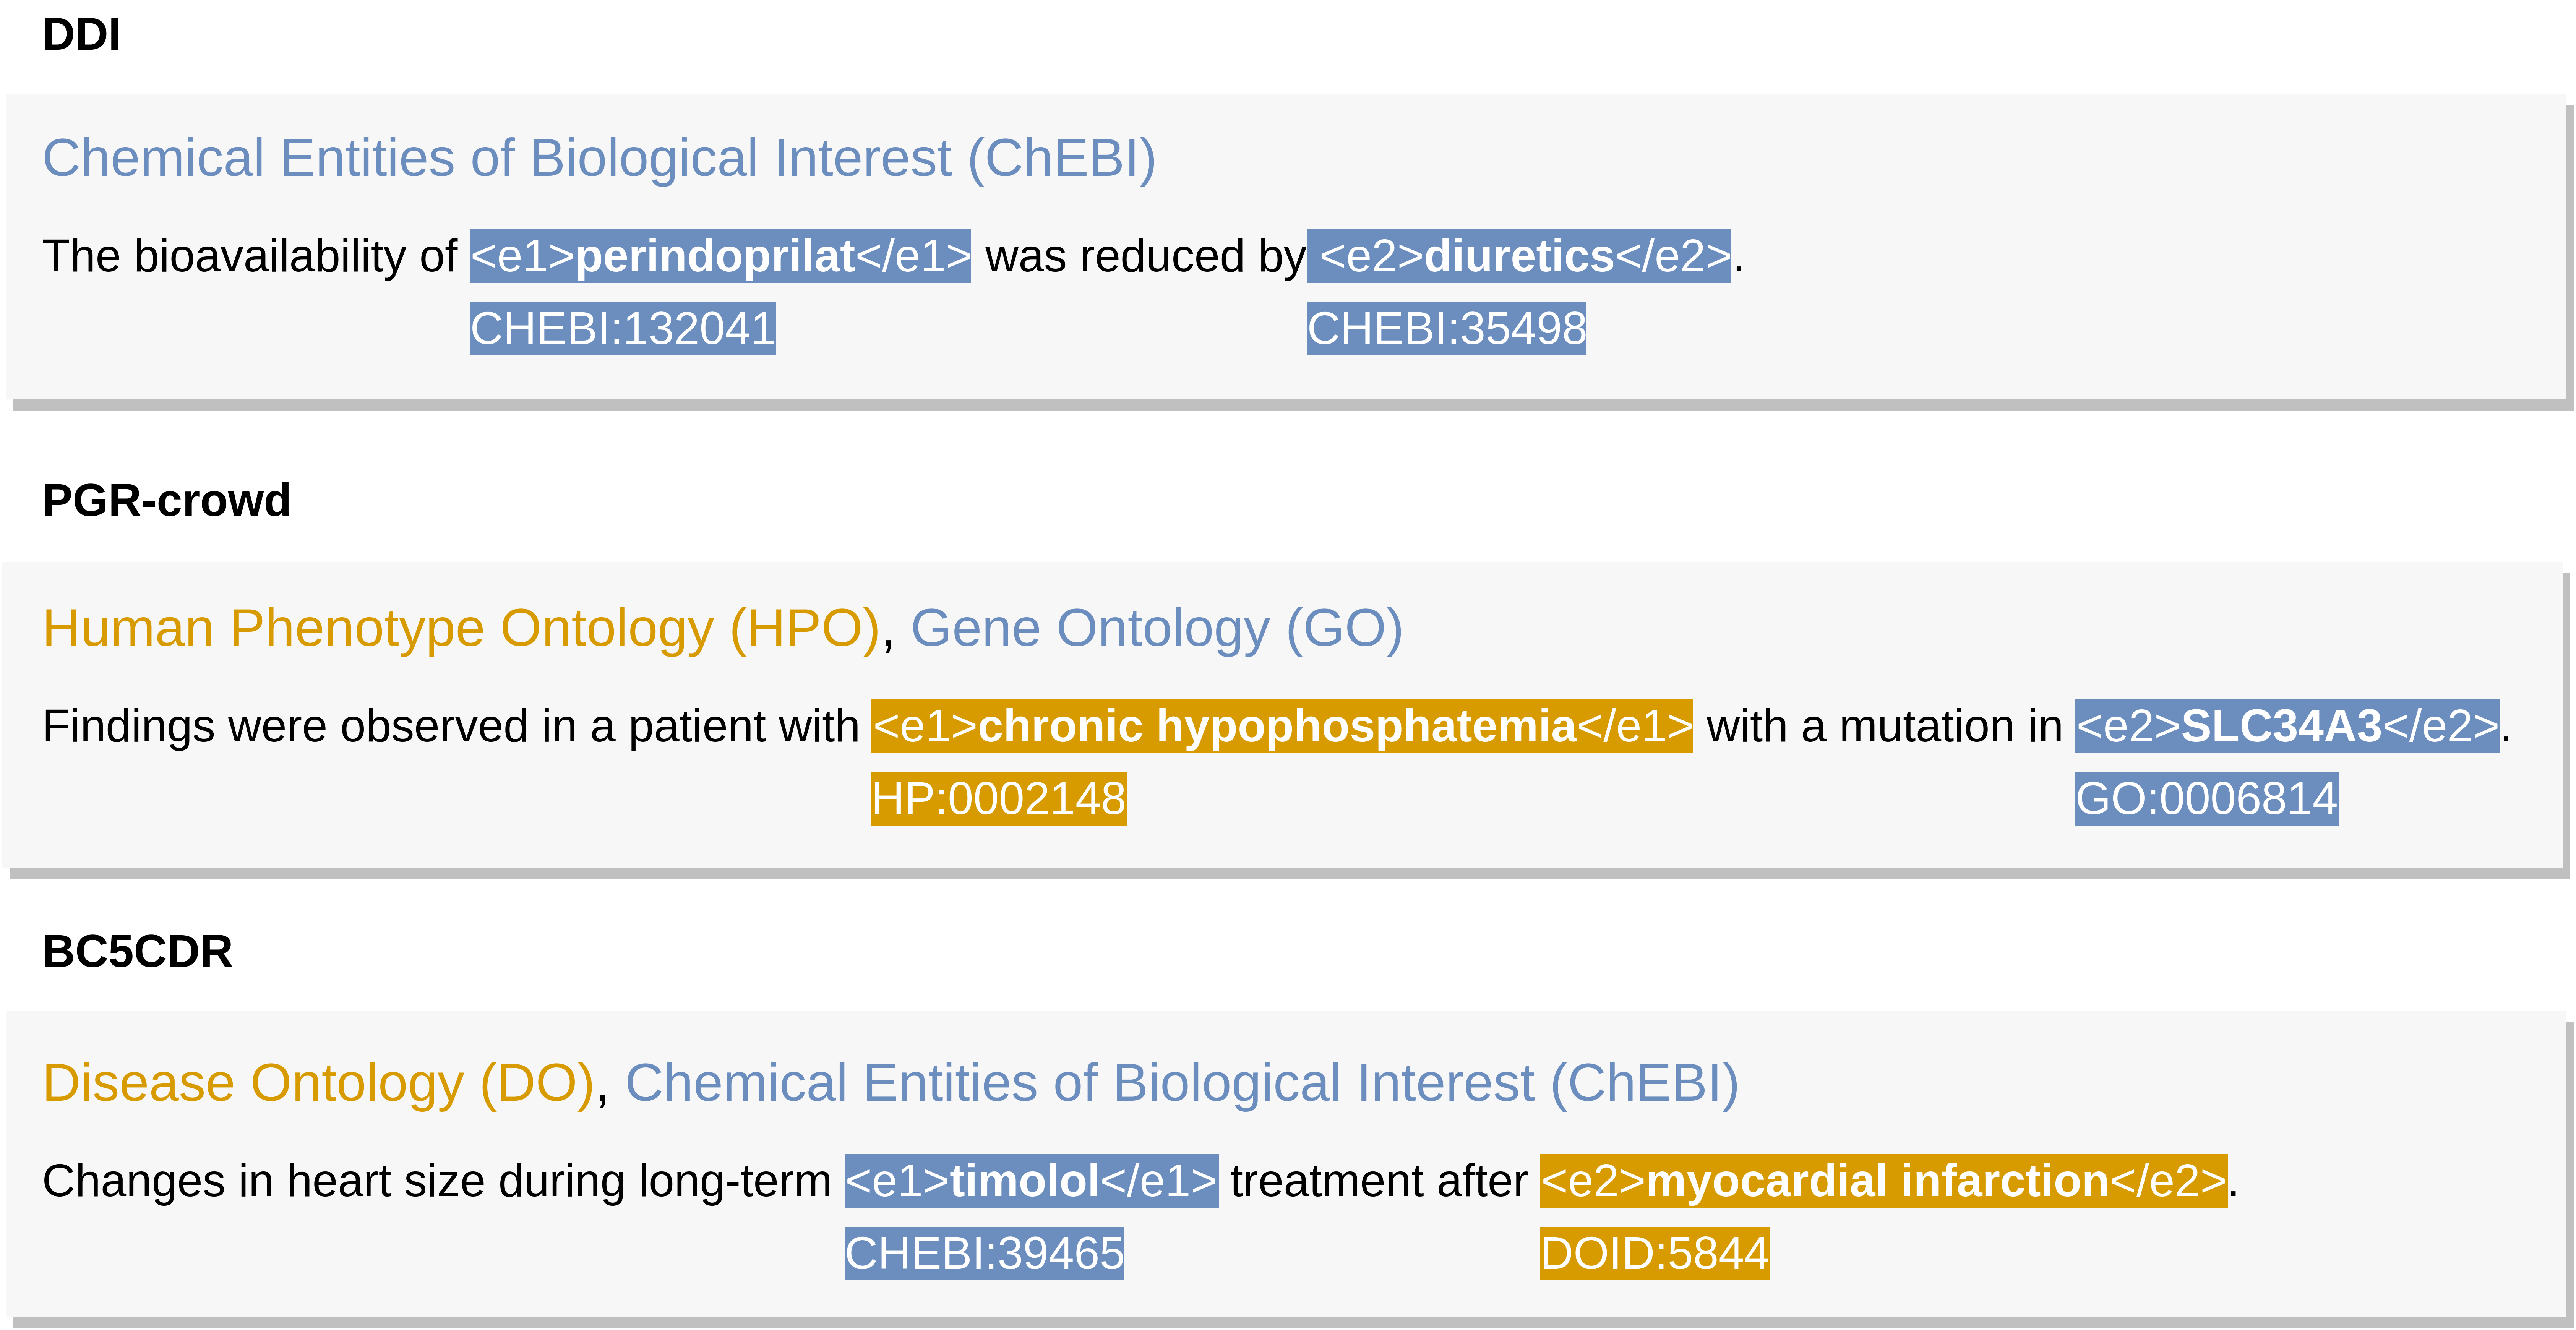
\includegraphics[width=\linewidth]{images/chapter_5/example_sentences_each_dataset.png}}
\caption[Three Sentence Examples for each dataset, DDI Corpus, PGR-crowd Corpus, and BC5CDR Corpus]{Three sentence examples for each dataset, DDI Corpus, PGR-crowd Corpus, and BC5CDR Corpus. The entities in each candidate relation are linked to corresponding knowledge bases.}\label{fig:52}
\end{figure}

We applied class weights to all datasets to normalize the different types of relations and distributions. Additionally, to train and evaluate all models on the same cross-validation splits, we split each dataset into training (60\%), validation (10\%), and test (30\%) sets. Also, our metrics presented below are displayed considering the weighted average for each type of relation to further account for the datasets' imbalances. 


\subsection{Knowledge Bases}

Several knowledge bases target biomedical entities, expanding on our information about them and their inherent relationships. Some of the knowledge bases or ontologies we can link to our target entities were mentioned above and are characterized in Table~\ref{Tab:02}\footnote{All knowledge bases were consulted on 20/04/2022}. 

\begin{table}[hbt!]
\centering
\caption[Main Characteristics of Biomedical Knowledge Bases]{The main characteristics of the following knowledge bases: Human Phenotype Ontology (HPO), Disease Ontology (DO), Chemical Entities of Biological Interest (ChEBI), and Gene Ontology (GO). All types of relations are transitive\label{Tab:02}} {\begin{tabular}{@{}lcp{3cm}p{5.5cm}@{}}\hline Knowledge bases &
Number of concepts & Type of relations & Specific characteristics\\\hline
HPO & 15670 & \textit{is-a} & Five sub-ontologies, from which \textit{phenotypic abnormality} is the most prevalent\\
DO & 13355 & \textit{is-a} & Human-specific\\
ChEBI & 153795 & \textit{is-a} & Refers to small molecular entities\\
 & & \textit{has-part} & \\
 & & \textit{is-conjugate-base-of} & \\
 & & \textit{is-conjugate-acid-of} & \\
 & & \textit{is-tautomer-of} & \\
 & & \textit{is-enantiomer-of} & \\
 & & \textit{has-functional-parent} & \\
 & & \textit{has-parent-hydride} & \\
 & & \textit{is-substituent-group-from} & \\
 & & \textit{has-role} & \\
GO & 43613 & \textit{is-a} & Three subontologies, molecular\\
 & & \textit{part-of} & function, biological process,\\
 & & \textit{has-part} & and cellular component\\
 & & \textit{regulates} & \\
 & & \textit{negatively-regulates} & \\
 & & \textit{positively-regulates} & \\\hline
\end{tabular}}
\end{table}

With few code adjustments, one can easily integrate more knowledge into K-RET in the form of other knowledge bases and has the flexibility to test different combinations swiftly.  


\subsection{Parameters and Training Details}

For each dataset, we empirically determined the best set of parameters. K-RET used a batch size of 32 for all datasets. The number of epochs ranged from 30 for DDI Corpus to 20 for PGR-crowd and BC5CDR Corpora (due to differences in dataset size). All other parameter settings were maintained from the original BERT model. The added knowledge only played a role in the fine-tuning and prediction stage.  

For the added knowledge, we varied the number of knowledge base entities allowed to link to each dataset entity in a candidate relation (or not). This variation ranged from two to five knowledge base entities per dataset entity. Our baseline represents the performance of the BERT-based systems without any added knowledge. When we refer to targeted knowledge, we mean just adding knowledge to entities in a candidate relation versus contextual knowledge, where we can add knowledge to all entities in the dataset. Figure \ref{fig:53} further elucidates the differences in the addition of knowledge. For the DDI Corpus, we used the ChEBI ontology; for the PGR-crowd, we used the HPO and the GO ontologies; and for the BC5CDR Corpus, we used the DO and ChEBI ontologies, as represented in Figure \ref{fig:52}.

\begin{figure*}[h]%figure3
\centerline{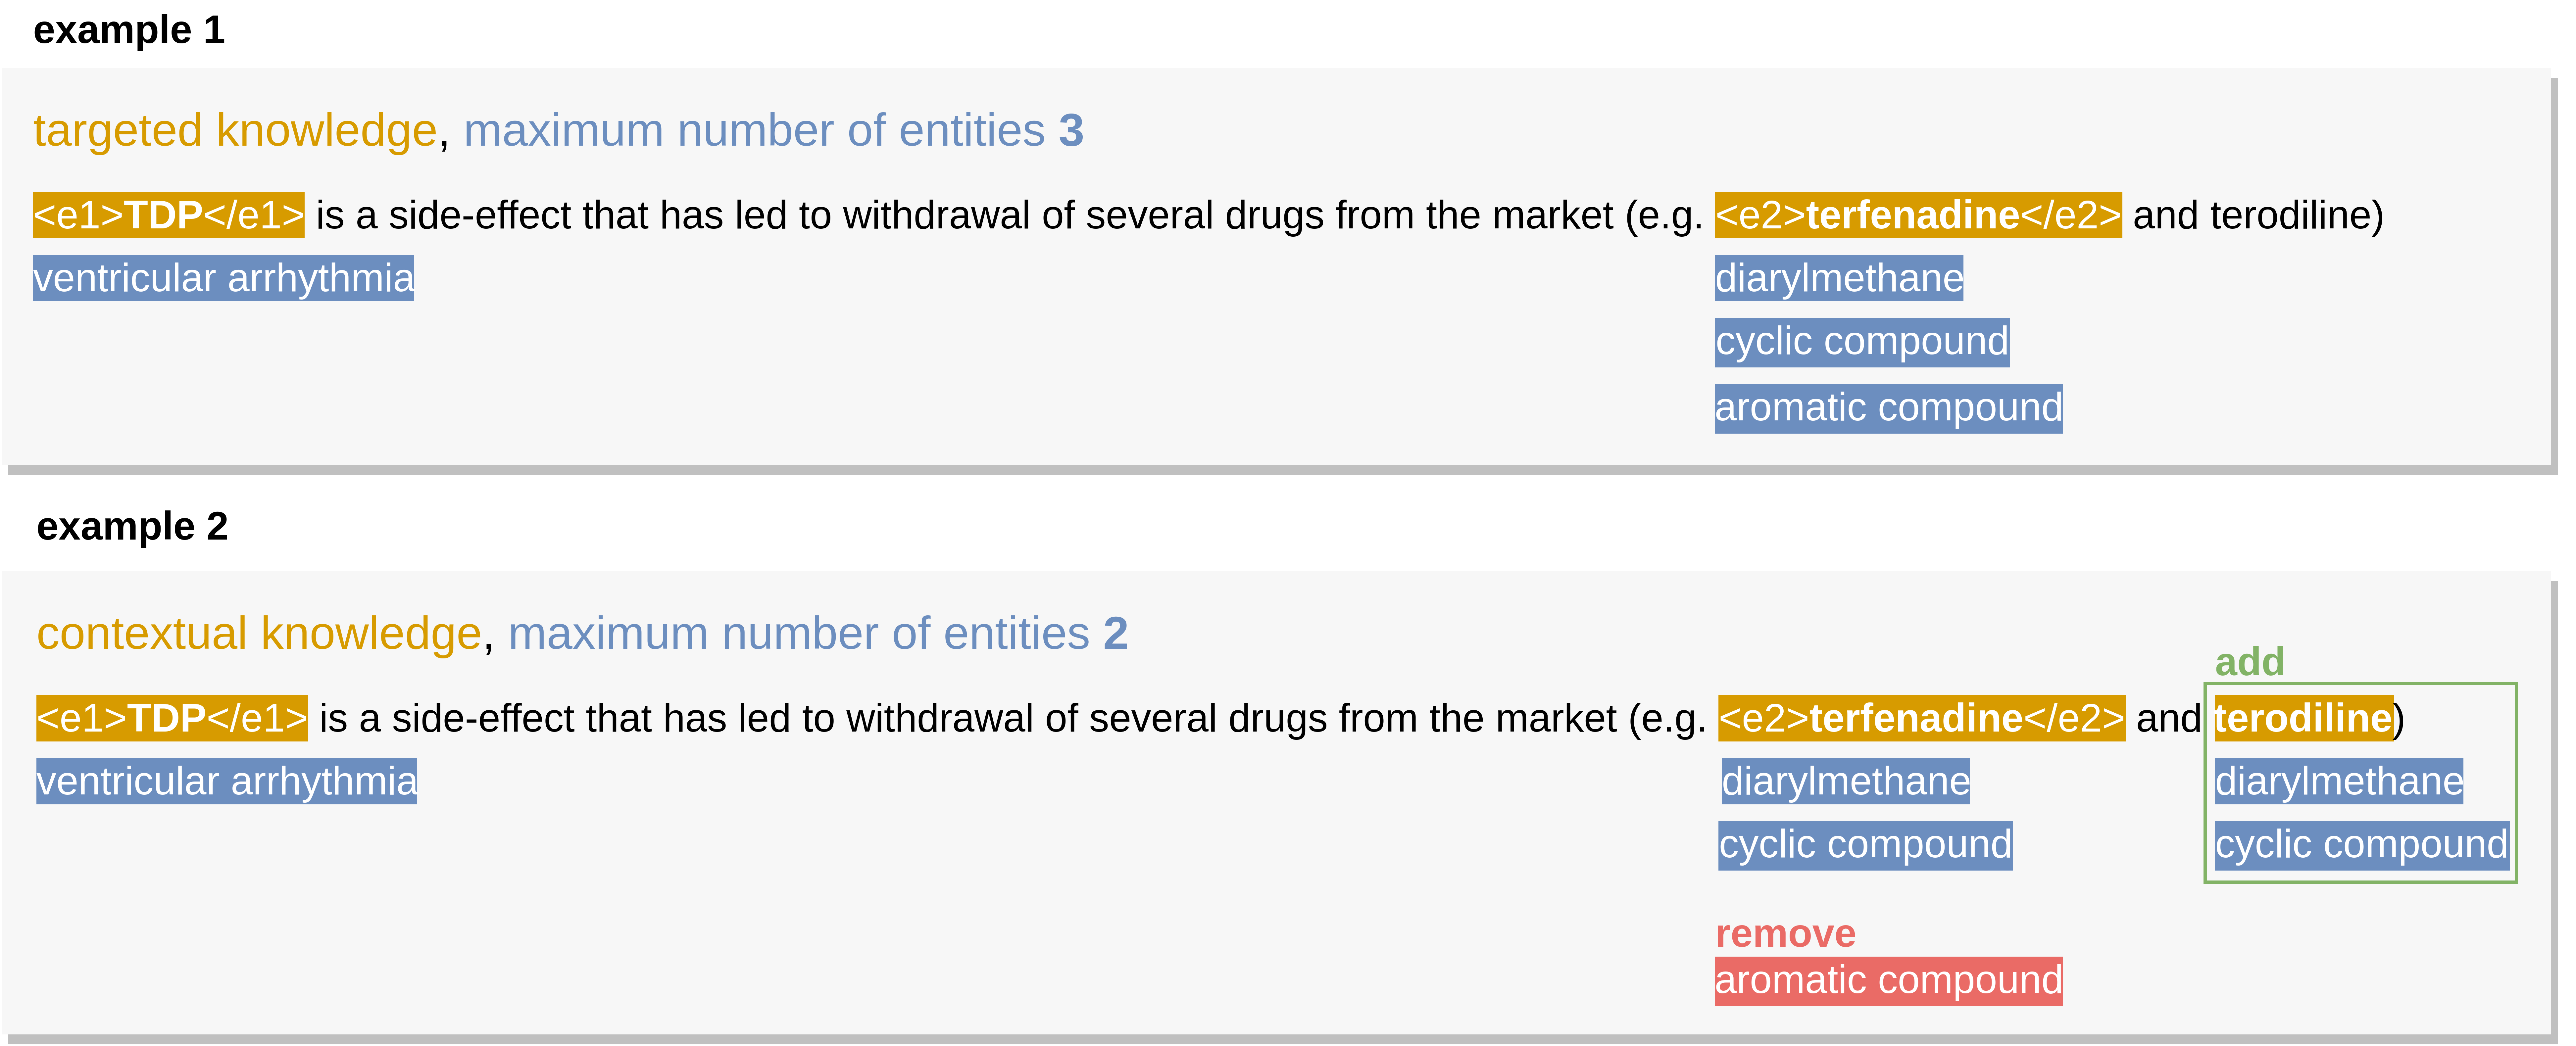
\includegraphics[width=\linewidth]{images/chapter_5/targeted_contextual_knowledge.png}}
\caption[Novelties of K-RET's Knowledge Injection Layer]{Novelties of K-RET's knowledge injection layer.  Example 1 presents a modality where we only add knowledge to entities in the candidate relation (targeted knowledge) and limit the number of knowledge base entities assigned to each entity (maximum number of entities 3). In example 2, we present the same sentence with the option of adding knowledge to all entities regardless if they are in the candidate relation (contextual knowledge) and limit the number of knowledge base entities assigned to each entity to two (maximum number of entities 2). From example 1 to example 2, we add a third knowledgeable entity (terodiline) and remove one of the knowledge base entities added (aromatic compound). The first entity can only be linked to one knowledge entity because (ventricular arrhythmia) no other association is established in the knowledge base.}\label{fig:53}
\end{figure*}

All models were trained on three Tesla M10 GPUs, taking, on average for each model, 24 hours (DDI Corpus), 1 hour (PGR-crowd Corpus), and 2 hours (BC5CDR Corpus). Each result presented in the following sections represents the averaged metrics for three runs except when it explicitly says otherwise, and each metric represents the weighted-averaged of the different labels.


\subsection{Results}

As mentioned in the previous sections, we divided our K-RET experiments into baseline, where we ran the BERT-based models without additional knowledge, targeted knowledge added to the entities in the candidate relation, and contextual knowledge added to all relevant entities in the sentence. We considered an entity relevant if present in the chosen knowledge source (i.e., a part of the domain knowledge considered). 

\subsubsection{Baseline}

To choose the best-performing BERT-based biomedical model for each of the three datasets, we used four of the most widely used systems: BERT \citep{devlin2019bert}, BioBERT \citep{lee2020biobert}, SciBERT \citep{scibert}, and PubMedBERT \citep{gu2021domain} integrated into K-BERT \citep{liu2020k} modified to perform RE. 

Table~\ref{Tab:03}\footnote{The specific models used were bert-base-uncased (BERT), scibert\_scivocab\_uncased (SciBERT), biobert-base-cased-v1.2 (BioBERT), BiomedNLP-PubMedBERT-base-uncased-abstract-fulltext (PubMedBERT)} reports the main results of testing the three datasets over the different BERT-based systems. For all three datasets, SciBERT is the best-performing system. Therefore, in our following experiments, we used SciBERT as the baseline system to which we added a knowledge layer.  

\begin{table}[h]
\centering
\caption[Baseline Performance of the Four Models for Each Dataset]{The baseline performance of the four models for each dataset\label{Tab:03}} 
\begin{tabular}{@{}llcccc@{}}\hline
Dataset & Model & Precision & Recall & F-measure & Accuracy\\\hline
PGR-crowd & BERT & 0.7247 & 0.7766 & 0.7332 & 0.7765\\
& SciBERT & \textbf{0.7680} & \textbf{0.8002} & \textbf{0.7462} & \textbf{0.7999}\\
& BioBERT & 0.6224 & 0.7888 & 0.6957 & 0.7888\\
& PubMedBERT & 0.7201 & 0.7834 & 0.7191 & 0.7833\\\hline
DDI & BERT & 0.7764 & 0.7798 & 0.7775 & 0.7796\\
& SciBERT & \textbf{0.7906} & \textbf{0.7964} & \textbf{0.7930} & \textbf{0.7960}\\
& BioBERT & 0.7796 & 0.7648 & 0.7680 & 0.7647\\
& PubMedBERT & 0.7801 & 0.7227 & 0.7473 & 0.7227\\\hline
BC5CDR & BERT & 0.5804 & 0.5614 & 0.5670 & 0.5615\\
& SciBERT & \textbf{0.6266} & \textbf{0.6364} & \textbf{0.6289} & \textbf{0.6363}\\
& BioBERT & 0.6150 & 0.6132 & 0.6142 & 0.6131\\
& PubMedBERT & 0.6091 & 0.6218 & 0.6113 & 0.6217\\\hline
\end{tabular}
\end{table}


\subsubsection{Targeted Knowledge}

For targeted knowledge, we added from two to five knowledge base entities to each entity in the candidate relation, as shown previously in example 1 (Figure \ref{fig:53}). Although we define the number of knowledge base entities to add, we are always limited by how many entities each entity is linked to in the knowledge base itself. Figure \ref{fig:54} presents the performance of the three datasets from no added knowledge (baseline) to five added entities per entity in the candidate relation.

Figure \ref{fig:54} shows that none of the K-RET models trained performs better than the baseline at any number of knowledge base added entities. For all datasets, there is a slight decrease in performance, with the BC5CDR Corpus having a small increase in performance when the number of added knowledge base entities equals three.  

\begin{figure}[H]
\centering
\begin{minipage}{0.48\textwidth}
\centering
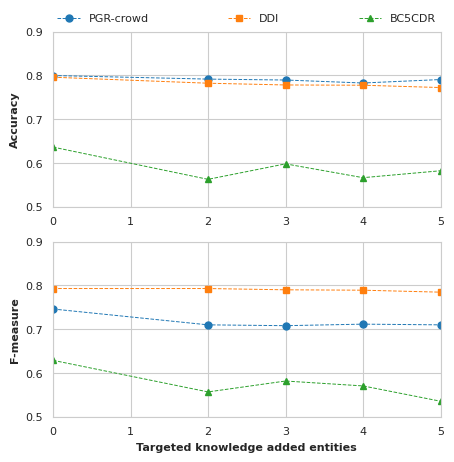
\includegraphics[width=0.97\linewidth]{images/chapter_5/tk.png}
\caption[K-RET Performance of the Targeted Knowledge Configuration]{The performance of the targeted knowledge K-RET configuration for the three datasets in Accuracy and F-Measure (top and bottom graphs, respectively) regarding the different number of added knowledge base entities.}\label{fig:54}
\end{minipage}
\hfill
\begin{minipage}{0.48\textwidth}
\centering
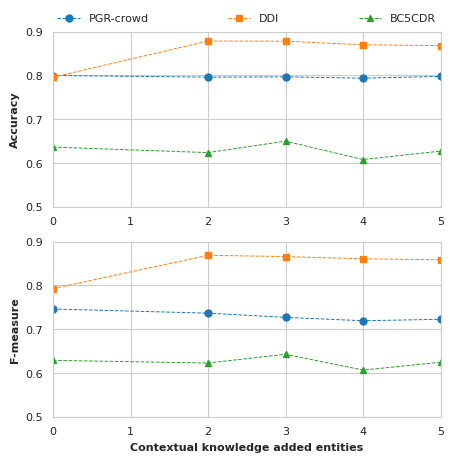
\includegraphics[width=0.97\linewidth]{images/chapter_5/ck.png}
\caption[K-RET Performance of the Contextual Knowledge Configuration]{The performance of the contextual knowledge K-RET configuration for the three datasets in Accuracy and F-Measure (top and bottom graphs, respectively) regarding the different number of added knowledge base entities.}\label{fig:55}
\end{minipage}
\end{figure}

\subsubsection{Contextual Knowledge}

We followed the same configuration mentioned above for contextual knowledge from two to five knowledge base entities added to each relevant entity in the sentence. Figure \ref{fig:55} presents the performance of the three datasets from no added knowledge (baseline) to five added entities per relevant entity. 

Figure \ref{fig:55} shows a performance increase from baseline to K-RET on the DDI and BC5CDR Corpora. For the PGR-crowd Corpus, while the performance is better than for targeted knowledge, the baseline performance still outperforms K-RET. Similarly, the BC5CDR's best performance is when the number of added knowledge base entities equals three, but this time surpasses the baseline. 

\vspace{10pt}
 
Table~\ref{Tab:04}\footnote{To facilitate table readability, we omitted the Standard Deviation (SD) values that range from 0.005 to 0.029 across all datasets due to the low impact these have on the interpretation of the final results.} presents the best results for each main model configuration (targeted and contextual), including the contextual knowledge configuration over ten runs to determine the statistical significance of the best configuration accurately and the corresponding baseline considered previously and regarding the majority label. The baseline\textsubscript{ML} represents the results if we assign the same label (majority label) to all the test relations. 

The results show that the contextual knowledge configuration over three runs prevails as the best model in two datasets (DDI and BC5CDR), with the targeted knowledge configuration not surpassing the baseline for any dataset. However, the BC5CDR Corpus presents a p-value of 0.8108 for F-measure and 0.8681 for accuracy ($\alpha = 0.05$), demonstrating a lack of significant difference between the means of Baseline and CK-RET\textsubscript{10}. Nonetheless, the DDI Corpus presents a p-value of $2.91 \times 10^{-12}$ for F-measure and $1.44 \times 10^{-12}$ for accuracy ($\alpha = 0.05$), validating a significant difference between the means of Baseline and CK-RET\textsubscript{10}. The p-values were determined using a one-tailed $t$-test.  

\begin{table}[h]
\centering
\caption[Final K-RET Performance Results]{The final K-RET performance results. The best-performing models for each dataset concerning baseline considering the majority label, baseline, targeted knowledge, contextual knowledge, and contextual knowledge over ten runs\label{Tab:04}} 
\begin{tabular}{@{}llcccc@{}}\hline
Dataset & Model & Precision & Recall & F-measure & Accuracy\\\hline
PGR-crowd & Baseline\textsubscript{ML} & 0.6222 & 0.7888 & 0.6957 & 0.7888\\
& Baseline & \textbf{0.7680} & \textbf{0.8002} & \textbf{0.7462} & \textbf{0.7999}\\
& TK-RET & 0.7891 & 0.7914 & 0.7100 & 0.7917\\
& CK-RET & 0.7614 & 0.7960 & 0.7367 & 0.7962\\\cline{2-6}

& CK-RET\textsubscript{10} & 0.7441 & 0.7933 & 0.7206 & 0.7934\\
\hline

DDI & Baseline\textsubscript{ML} & 0.7267 & 0.8525 & 0.7846 & 0.8525\\
& Baseline & 0.7906 & 0.7964 & 0.7930 & 0.7960\\
& TK-RET & 0.8132 & 0.7820 & 0.7930 & 0.7823\\
& CK-RET & 0.8674 & 0.8791 & 0.8690 & 0.8788\\\cline{2-6}

& CK-RET\textsubscript{10} & \textbf{0.8704} & \textbf{0.8805} & \textbf{0.8719} & \textbf{0.8804} \\\hline

BC5CDR & Baseline\textsubscript{ML} & 0.3803 & 0.6167 & 0.4705 & 0.6167\\
 & Baseline & 0.6266 & 0.6364 & 0.6289 & 0.6363\\
& TK-RET & 0.5838 & 0.5977 & 0.5816 & 0.5980\\
& CK-RET & \textbf{0.6412} & \textbf{0.6499} & \textbf{0.6428} & \textbf{0.6498}\\\cline{2-6}

\rule{0pt}{3.2ex} & CK-RET\textsubscript{10} & 0.6317 & 0.6348 & 0.6309 & 0.6347 \\\hline
\end{tabular}
\end{table}

Table~\ref{Tab:05} reflects the specific performance of the DDI Corpus per type of relation (\textit{effect}, \textit{advice}, \textit{mechanism}, \textit{int}, and \textit{false}) for each main model configuration. Table A1 and Table A2 in Supplementary Data present the same results for PGR-crowd and BC5CDR Corpora. For the DDI Corpus, we also performed ablation regarding multi-token entities by limiting the association of knowledge to the first entity within the multi-token considered. We obtained an F-measure of 0.8663 and an accuracy of 0.8732.    

\begin{table}[h]
\centering
\caption[DDI Corpus Performance per Type of Relation]{DDI Corpus performance per type of relation\label{Tab:05}} 
\begin{tabular}{@{}llccccc@{}}
\hline \multirow{2}{*}{Metrics} & \multirow{2}{*}{Model} &
\multicolumn{5}{c}{Type} \\\cline{3-7}
& & Effect & Advice & Mechanism & Int & False\\\hline
Precision & Baseline & 0.1770 & 0.0890 & 0.2720 & 0.2800 & 0.8060\\
& TK-RET & 0.2747 & 0.3053 & 0.3623 & 0.2360 & 0.9020 \\
& CK-RET & 0.5137 & \textbf{0.6720} & \textbf{0.5757} & 0.5963 & 0.9163 \\\cline{2-7}

& CK-RET\textsubscript{10} & \textbf{0.5524} & 0.6370 & 0.5411 & \textbf{0.6659} & \textbf{0.9194} \\
\hline
Recall & Baseline & 0.2000 & 0.0730 & 0.1810 & 0.3850 & 0.9040\\
& TK-RET & 0.4677 & 0.3490 & 0.5127 & 0.0160 & 0.8487 \\
& CK-RET & 0.4533 & 0.2937 & 0.4950 & \textbf{0.4340} & \textbf{0.9600} \\\cline{2-7}

& CK-RET\textsubscript{10} & \textbf{0.4758} & \textbf{0.3226} & \textbf{0.5318} & 0.3946 & 0.9579\\
\hline
F-measure & Baseline & 0.1880 & 0.0800 & 0.2170 & 0.3250 & 0.9000\\
& TK-RET & 0.3423 & 0.3240 & 0.4187 & 0.0293 & 0.8743 \\
& CK-RET & 0.4810 & 0.4077 & 0.5317 & \textbf{0.5017} & 0.9377 \\\cline{2-7}

& CK-RET\textsubscript{10} & \textbf{0.5099} & \textbf{0.4266} & \textbf{0.5329} & 0.4924 & \textbf{0.9384}\\
\hline
\end{tabular}
\end{table}


\section{Discussion}

From the experiences conducted throughout the previous section, we can infer that adding knowledge can significantly improve the state-of-the-art performance of one of the most used biomedical Relation Extraction (RE) datasets, mainly when using contextual knowledge. However, there is a difference in how significantly we can improve performance, from nothing (PGR-crowd Corpus) to over 0.076 percentage points (DDI Corpus). Several factors can explain the differences in performance for the different datasets, such as dataset size and label distribution, knowledge base size and coverage of the dataset entities, or the average number of knowledge base entities that can be linked to each dataset entity.

For the PGR-crowd Corpus, while all entities are linked to one of two knowledge bases, the Human Phenotype Ontology (HPO) or the Gene Ontology (GO), the linking to the GO is already second-handed. In the PGR-crowd Corpus, the authors recognized gene entities and posteriorly linked them to their most representative GO term. We do not use their gene identifiers directly because these biomedical entities are not directly represented in any hierarchic knowledge base. Thus, we used the GO terms to add further information and, consequently, distanced ourselves from the original gene entity. However, what made the most significant impact in the lack of increase in performance is the distribution of labels being predominantly \textit{true}. Identifying undetected \textit{true} relations is more challenging than if the dataset was more balanced (e.g., the BC5CDR Corpus) or with the inverse distribution (e.g., the DDI Corpus). Also, for the specific case of PGR-crowd Corpus, there could be ambiguity if an acronym describes a human phenotype or a gene since these can often overlap. This ambiguity is an open problem, and in this work, we opted not to consider human phenotype entities acronyms for contextual knowledge, which could be made us lose valuable information.   

With the BC5CDR Corpus, K-RET only surpassed the baseline when adding contextual knowledge by slightly over 1\% in both F-measure and accuracy and was unsuccessful at demonstrating a significant difference between the baseline and the best-performing configuration. Although the impact on performance is not preeminent, the fact that this dataset is denser in the number of relevant entities per sentence and more evenly distributed than the PGR-crowd Corpus increases the impact of the addition of knowledge. This behaviour occurs when knowledge is added directly to the candidate relation's target entities and peripherally to other relevant entities. 

The DDI Corpus is unbalanced in favour of \textit{no\_relation}/\textit{false} labels. Therefore, finding \textit{true} relations is more challenging. This dataset's distribution of labels is ideal for increasing the impact of adding knowledge. The label distribution, the highly dense text in relevant entities, and the ampler size of the knowledge base used, Chemical Entities of Biological Interest (ChEBI), all contribute to the rise in performance by adding contextual knowledge. The improvements from baseline were 7.60\% for contextual knowledge in F-measure. We also verified that adding knowledge made a bigger impact on system performance than using multi-token entities by contributing to an average improvement of 0.0704 data points in F-measure and 0.0756 in accuracy. 

K-RET was able to design a more efficient and flexible knowledge layer than the previous attempt in the work of \cite{liu2020k} by applying knowledge injection to the biomedical RE task. First, by proving the utility of contextualizing tokens, with substantial improvements in one of the three datasets described above from targeted to contextual token usage. Second, by the possibility of adding more than one knowledge source to cover the domains of all relevant entities mentioned in the training data. Third, by incorporating the option of adding knowledge to multi-token entities instead of only single-token. We determined experimentally for the DDI Corpus the multi-token approach to be more thorough, which can be explained by those entities constituting the majority of biomedical entities described in the datasets used for testing.

\section{Conclusion}

This paper proposed a new biomedical Relation Extraction (RE) system, K-RET, that incorporates knowledge in the form of ontologies into BERT-based systems to enrich and complement the data used for training. K-RET is a flexible system that can handle different associations, integrate knowledge from multiple sources, define where to apply the knowledge, and deal with multi-token entities. We used three independent and open-access RE datasets to test our system concerning different types of biomedical entities with different characteristics (i.e., label distribution). Allied with the three datasets, we used four knowledge bases to inject knowledge according to the type of entities involved in the candidate relations. The best-performing dataset was the DDI Corpus allied with the Chemical Entities of Biological Interest (ChEBI) knowledge base, with significant average improvements compared with the baseline in the order of 7.60\% and 8.28\% for F-measure and accuracy, respectively. For the BC5CDR Corpus, we also had modest improvements (an average of 1.39\% and 1.35\% for F-measure and accuracy), even though we did not find these results significant. Differently, for the PGR-crowd Corpus, there was no significant change in performance from the addition of knowledge. Thus, we concluded that the label distribution and relevant entity density within the training data significantly affect how our system performs. Nevertheless, we successfully demonstrated the power of adding external knowledge to training data and how to accommodate it to different domain data. 

In a nutshell, the K-RET system successfully added contextual knowledge, more than one knowledge source, and knowledge to multi-token entities. 

For future work, we would like to explore the impact of different knowledge bases and combinations within the ones we already used. Also, we would like to analyze further and examine the implications of peripherical contextual entities on assigning a label for a candidate relation and entities overlapping within different knowledge bases. 
